% ============================================================================================
% BAB III ANALISIS MASALAH
% Pembagian subbab tidak rigid dan dapat bervariasi. Bab ini minimal berisi analisis kebutuhan
% fungsional dan nonfungsional, analisis berbagai alternatif solusi yang dapat ditawarkan, dan
% metode pemilihan solusi yang diusulkan.
% ============================================================================================
\chapter{ANALISIS MASALAH}
\label{chap:analisis-masalah}

\section{Analisis Kondisi Saat Ini}
Bagian ini menjelaskan kondisi saat ini terkait bagaimana \textit{spyware} 
tradisional melakukan proses mulai dari infeksi, pengambilan data, hingga 
eksfiltrasi. Alur kerja \textit{spyware} saat ini digunakan sebagai dasar 
untuk memahami pola kerja \textit{spyware} yang ada saat ini.

\begin{figure}[H]
    \centering
    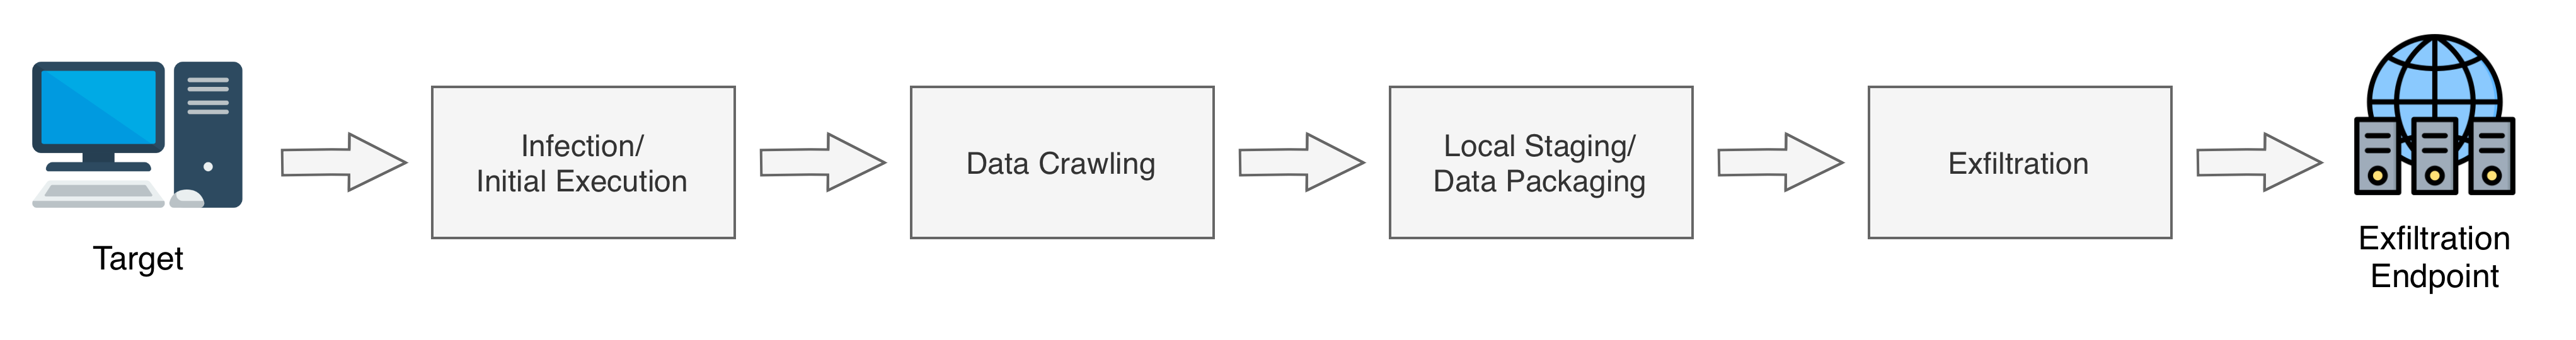
\includegraphics[width=\textwidth]{image/kondisi-saat-ini.png}
    \caption{Alur Kerja \textit{Data Crawling} dan Eksfiltrasi \textit{Spyware} Saat Ini}
    \label{fig:alur-spyware}
\end{figure}

Gambar \ref{fig:alur-spyware} menggambarkan alur kerja umum \textit{spyware} 
dalam melakukan pengambilan dan pengiriman data dari perangkat target. 
Proses dimulai dari tahap infeksi atau eksekusi awal, ketika \textit{spyware} 
berhasil dijalankan di dalam sistem target dan menempatkan dirinya. 
Setelah aktif, \textit{spyware} memulai tahap \textit{data crawling}, yaitu 
proses pengumpulan data secara otomatis dan sistematis terhadap berbagai 
informasi sensitif. Data yang terkumpul kemudian tidak langsung dikirimkan, 
melainkan diproses terlebih dahulu melalui \textit{local staging}, misalnya 
dengan kompresi, enkripsi, atau pemecahan data ke dalam paket kecil agar lebih 
mudah disamarkan. 
Tahap selanjutnya adalah eksfiltrasi, yaitu proses pengiriman data yang telah 
dipaketkan menuju infrastruktur penyerang melalui kanal komunikasi tertentu. 
Setelah itu data mencapai \textit{exfiltration endpoint}.

\subsection{Tantangan \textit{Data Crawling} dan Eksfiltrasi \textit{Spyware}}
Dalam melakukan \textit{data crawling} dan eksfiltrasi, ada beberapa tantangan yang dihadapi oleh \textit{spyware}:

\begin{enumerate}
    \item Aktivitas \textit{crawling} yang \textit{high noise} dan mudah terpantau \\
    Aktivitas \textit{crawling} yang berjalan secara intensif tanpa pengendalian frekuensi dapat menghasilkan pola akses file, direktori, dan API yang berulang sehingga memunculkan \textit{high-noise behavior} yang mudah terdeteksi oleh sistem keamanan berbasis perilaku. Menurut studi deteksi \textit{malware} berbasis \textit{system call} dan \textit{file I/O}, frekuensi akses file serta urutan \textit{system call} yang tidak lazim merupakan indikator kuat proses berbahaya, sehingga pola \textit{crawling} yang padat berpotensi terbaca sebagai anomali meskipun tidak bersifat \textit{malicious} \autocite{chukwuani2025mltechniques}.

    \item Risiko deteksi dari pola akses yang intensif \\
    \textit{Crawling} yang melibatkan pembacaan file, pemindaian direktori, atau interaksi API dalam frekuensi tinggi dapat menimbulkan pola aktivitas yang berbeda dari aplikasi normal. Temuan pada penelitian \textcite{sheen2022rsentry} menunjukkan bahwa sistem deteksi berbasis perilaku memanfaatkan penyimpangan pola akses file tersebut, misalnya dengan mengidentifikasi lonjakan jumlah \textit{file accesses} dalam interval waktu tertentu atau mendeteksi urutan \textit{directory traversal} yang tidak lazim.

    \item Eksfiltrasi melalui kanal standar yang mudah dipantau \\
    Pengiriman data oleh malware maupun \textit{spyware} sering memanfaatkan protokol umum karena protokol tersebut biasanya diizinkan dan menjadi bagian dari trafik normal jaringan. Namun, penelitian \textcite{ullah2018dataexfiltration} menunjukkan bahwa meskipun kanal-kanal ini bersifat sah, pola eksfiltrasi yang tidak disamarkan tetap dapat terdeteksi ketika karakteristik komunikasinya tidak menyerupai perilaku aplikasi \textit{benign}. Mekanisme seperti \textit{known-channel inspection} dan \textit{anomaly-based detection} dapat mengidentifikasi eksfiltrasi melalui pemeriksaan konteks trafik, termasuk frekuensi, ukuran, konten, dan format paket, serta membandingkannya dengan pola penggunaan wajar.

    \item Pola eksfiltrasi yang kasar atau bulk transfer \\
    Pola eksfiltrasi yang mengirimkan data dalam jumlah besar sekaligus atau menggunakan interval pengiriman yang tetap cenderung menghasilkan jejak komunikasi yang seragam dan tidak dinamis. Menurut \textcite{sabir2021mldetect}, sistem deteksi berbasis \textit{machine learning} dapat mengidentifikasi anomali dengan mempelajari pola komunikasi normal, termasuk variasi ukuran \textit{payload}, frekuensi pengiriman, dan distribusi data dalam trafik sehari-hari. Studi tersebut menjelaskan bahwa deviasi seperti pengiriman file berukuran besar secara tiba-tiba atau pola transfer yang konsisten dan berulang akan langsung dibedakan dari perilaku \textit{benign}, karena komunikasi normal umumnya menunjukkan variasi ukuran, timing, dan volume.
\end{enumerate}

\subsection{\textit{Gap Analysis}}
Pada bagian ini disajikan \textit{gap analysis} yang mengidentifikasi perbedaan antara kondisi saat ini (\textit{As-Is}) dan kondisi ideal (\textit{To-Be}) terkait kemampuan pengumpulan data (\textit{crawling}) dan proses eksfiltrasi. Tabel~\ref{tbl:gap-analysis} merangkum domain masalah utama, observasi kondisi saat ini, kesenjangan yang teridentifikasi, serta kondisi ideal yang menjadi sasaran perbaikan.
\begin{table}[H]
\captionsetup{justification=raggedright,singlelinecheck=false}
\centering
\caption{\textit{Gap Analysis}}
\label{tbl:gap-analysis}
\begin{tabular}{|p{2.7cm}|p{3.5cm}|p{3.5cm}|p{3.5cm}|}
\hline
\textbf{Domain Masalah} &
\textbf{Kondisi Saat Ini (\textit{As-Is})} &
\textbf{Kesenjangan (\textit{Gap})} &
\textbf{Kondisi Ideal (\textit{To-Be})} \\
\hline

Aktivitas \textit{crawling} &
Proses \textit{crawling} dijalankan dari \textit{executable} di disk dan menggunakan akses file/direktori untuk mengambil data, sehingga meninggalkan artefak. &
Belum ada mekanisme untuk meminimalkan jejak \textit{crawling}. &
\textit{Crawling} dilakukan dengan jejak minimal melalui \textit{in-memory processing}, penghapusan \textit{buffer} otomatis per \textit{batch}, dan tanpa meninggalkan artefak yang mudah terdeteksi di disk. \\
\hline

Kanal eksfiltrasi dan karakteristik trafik &
Eksfiltrasi menggunakan protokol umum tetapi pola trafik tidak disamarkan dan tetap mudah dibedakan dari komunikasi aplikasi sah. &
Kanal komunikasi belum menyerupai trafik normal dan karakteristik paket belum tersamarkan sehingga aktivitas dapat terdeteksi. &
Eksfiltrasi berlangsung melalui kanal yang menyerupai trafik sah dengan pola komunikasi adaptif, terenkripsi, dan tidak mencolok. \\
\hline

Mekanisme eksfiltrasi &
Data hasil \textit{crawling} langsung dikirim ke \textit{endpoint} tanpa enkripsi atau kompresi khusus, sehingga struktur \textit{payload} masih mudah diinterpretasi. &
Tidak ada mekanisme untuk mengamankan \textit{payload} eksfiltrasi. &
Eksfiltrasi dilakukan dengan \textit{payload} terenkripsi, dikemas, atau disamarkan sehingga tidak mudah dibaca maupun dianalisis. \\
\hline

\end{tabular}
\end{table}


\section{Analisis Kebutuhan}
\subsection{Identifikasi Masalah Pengguna}

Kelompok pengguna utama yang memanfaatkan hasil pengujian kapabilitas deteksi antivirus terhadap \textit{spyware} mode \textit{stealth} terdiri atas tiga kelompok: peneliti keamanan siber, pengembang \textit{malware} uji, dan penyedia antivirus. Ketiganya berperan penting dalam memastikan proses pengembangan, pengujian, serta analisis hasil deteksi berjalan aman, terkendali, dan memberikan hasil yang valid.

\begin{enumerate}
    \item Peneliti Keamanan Siber \\
    Kelompok ini memanfaatkan hasil pengujian untuk mengevaluasi efektivitas mekanisme deteksi terhadap ancaman \textit{spyware} dengan mode \textit{stealth} serta mengidentifikasi celah-celah deteksi yang masih ada. Temuan dari penelitian ini digunakan sebagai dasar pembuatan rekomendasi teknis dan strategi penguatan sistem pertahanan dengan tujuan meningkatkan kemampuan deteksi dan respons terhadap skenario pengumpulan data (\textit{data crawling}) dan eksfiltrasi yang bersifat tersembunyi.

    \item Pengembang \textit{Malware} Uji \\
    Kelompok ini bertugas membangun \textit{spyware} dengan mode \textit{stealth} yang meniru perilaku nyata, terutama pada tahap \textit{data crawling} dan eksfiltrasi. Tantangan utama mereka adalah mengimplementasikan perilaku pengumpulan dan pengiriman data secara tersembunyi tanpa menyebabkan kerusakan nyata maupun terdeteksi terlalu dini oleh antivirus. Selain itu, pengembang harus memastikan keamanan lingkungan uji agar \textit{malware} tidak keluar dari batas laboratorium.

    \item Penyedia Antivirus atau EDR \\
    Penyedia antivirus atau EDR menjadi pengguna yang memperoleh manfaat praktis dari hasil penelitian berupa bukti empiris terkait \textit{blindspot} produk, rekomendasi konfigurasi telemetri, dan \textit{scenario-driven test cases}. Informasi ini dapat digunakan untuk memperbaiki aturan deteksi, menambah cakupan pengumpulan telemetri, serta meningkatkan kebijakan respons insiden sehingga produk lebih tangguh terhadap varian \textit{stealth} yang berkembang.
\end{enumerate}

\subsection{Kebutuhan Fungsional}

Kebutuhan fungsional merupakan spesifikasi yang mendefinisikan fitur-fitur inti 
yang harus disediakan oleh \textit{malware} uji agar dapat memenuhi tujuan dalam 
proses penelitian dan pengembangan. Kebutuhan ini dirancang untuk memastikan 
setiap kemampuan utama dapat dijalankan secara efektif dalam lingkungan uji 
sesuai skenario penelitian.

\begin{longtable}{|p{1.5cm}|p{5cm}|p{7cm}|}
\caption{Kebutuhan Fungsional}
\label{tbl:kebutuhan-fungsional} \\
\hline
\textbf{ID} & \textbf{Kebutuhan} & \textbf{Penjelasan} \\
\hline
\endfirsthead

\hline
\textbf{ID} & \textbf{Kebutuhan} & \textbf{Penjelasan} \\
\hline
\endhead

\hline
\endfoot

FR-01 &
Sistem dapat melakukan proses \textit{crawling} data secara \textit{stealth} &
Sistem harus memfasilitasi metode \textit{crawling} bertahap (\textit{low and slow}), 
memanfaatkan proses atau API sah (\textit{living off the land}) agar pola akses menyerupai aktivitas normal 
sehingga sulit terdeteksi \textit{anti-malware}. \\
\hline

FR-02 &
Sistem mendukung eksfiltrasi data menggunakan metode yang sulit dianalisis &
Eksfiltrasi dilakukan melalui kanal terenkripsi, 
data dicicil secara acak, serta menyamarkan trafik sehingga tidak mudah dibedakan dari aktivitas jaringan normal oleh deteksi keamanan. \\
\hline

FR-03 &
Sistem tidak menyimpan artefak proses \textit{crawling} atau eksfiltrasi di disk &
Semua proses berjalan \textit{in-memory}, tanpa membuat file \textit{temporary} yang dapat dianalisis secara forensik, 
serta mendukung \textit{memory wiping} setelah selesai eksekusi. \\
\hline

FR-04 &
Sistem memungkinkan penyembunyian aktivitas \textit{crawling} dan eksfiltrasi dalam proses aplikasi sah &
Aktivitas bisa disisipkan melalui teknik \textit{injection/hollowing} ke aplikasi yang dipercaya, 
agar \textit{event crawling} dan eksfiltrasi tersamarkan sebagai aktivitas aplikasi legal. \\
\hline

FR-05 &
Sistem dapat melakukan \textit{clean up} otomatis untuk menghilangkan jejak digital &
Setelah aktivitas \textit{crawling} dan eksfiltrasi selesai, sistem menghapus artefak, jejak \textit{log}, atau \textit{payload} sementara 
sehingga \textit{anti-malware} maupun forensik tidak menemukan indikasi aktivitas berbahaya. \\
\hline

\end{longtable}

\subsection{Kebutuhan Non-Fungsional}
Kebutuhan non-fungsional mendefinisikan karakteristik kualitas, batasan, dan 
standar yang harus dipenuhi oleh \textit{malware} uji selama pelaksanaan 
eksperimen. Kebutuhan ini berfokus pada aspek keamanan, kepatuhan, efisiensi, 
serta dampak perilaku \textit{malware} di lingkungan pengujian untuk memastikan 
penelitian berjalan dengan aman, terkendali, dan sesuai prinsip etika akademik.

\begin{longtable}{|p{1.5cm}|p{5cm}|p{7cm}|}
\caption{Kebutuhan Non-Fungsional}
\label{tbl:kebutuhan-nonfungsional} \\
\hline
\textbf{ID} & \textbf{Kebutuhan} & \textbf{Penjelasan} \\
\hline
\endfirsthead

\hline
\textbf{ID} & \textbf{Kebutuhan} & \textbf{Penjelasan} \\
\hline
\endhead

\hline
\endfoot

NFR-01 & Kinerja &
Sistem harus mampu melakukan \textit{crawling} dan eksfiltrasi data tanpa menimbulkan konsumsi
\textit{resource} (CPU, memori, jaringan) yang tinggi agar tidak memicu alarm \textit{anti-malware}
atau monitoring forensik. \\
\hline

NFR-02 & Reliabilitas &
Segala \textit{failure} harus ditangani secara \textit{silent} (tidak menimbulkan pesan
\textit{error}/\textit{alert} pada \textit{endpoint} atau sistem keamanan). \\
\hline

NFR-03 & Keamanan lingkungan uji &
Sistem harus memastikan seluruh eksekusi \textit{malware} berlangsung dalam lingkungan yang benar-benar terisolasi dan tidak terhubung dengan sistem produksi. \\
\hline

NFR-04 & Kepatuhan terhadap regulasi dan etika penelitian &
Sistem wajib mematuhi regulasi keamanan siber, etika penelitian, serta tidak menggunakan
\textit{malware} untuk tujuan di luar pengujian akademik terisolasi. \\
\hline

NFR-05 & Isolasi Dampak &
Efek dan aktivitas \textit{malware} harus benar-benar terbatas pada lingkungan uji,
tidak boleh berdampak pada sistem luar sehingga integritas lab tetap terjaga. \\
\hline

\end{longtable}

\section{Analisis Pemilihan Solusi }
\subsection{Alternatif Solusi}

Permasalahan yang ditemukan dalam penelitian ini perlu dianalisis secara menyeluruh agar arah penyusunan solusi menjadi lebih terarah dan relevan dengan tujuan penelitian. Hasil identifikasi terhadap berbagai kendala yang muncul selama tahap studi literatur dan observasi awal kemudian dirangkum dalam Tabel~\ref{tbl:masalah-dampak}. Tabel tersebut memuat daftar masalah utama beserta dampaknya terhadap proses \textit{data crawling} dan eksfiltrasi dalam rangka menguji kapabilitas deteksi \textit{anti-spyware} yang ada saat ini.

\begin{longtable}{|c|p{6cm}|p{6.2cm}|}
\caption{Masalah dan Dampak}
\label{tbl:masalah-dampak} \\
\hline
\textbf{ID} & \textbf{Masalah} & \textbf{Dampak} \\
\hline
\endfirsthead

\hline
\textbf{ID} & \textbf{Masalah} & \textbf{Dampak} \\
\hline
\endhead

\hline
\endfoot

M-01 &
Proses \textit{crawling} dijalankan dari \textit{executable} di disk sehingga meninggalkan artefak. &
Artefak di disk dapat dideteksi melalui \textit{signature-based scanning}. \\
\hline

M-02 &
Pola akses sistem yang tidak sesuai \textit{baseline} dapat terdeteksi sebagai aktivitas abnormal. &
Aktivitas \textit{crawling} lebih mudah teridentifikasi oleh deteksi berbasis perilaku, sehingga menurunkan tingkat \textit{stealth}. \\
\hline

M-03 &
Eksfiltrasi melalui protokol umum tanpa penyamaran pola trafik. &
\textit{Anti-spyware} dapat mendeteksi anomali trafik, sehingga proses eksfiltrasi berisiko terblokir atau memicu alarm. \\
\hline

M-04 &
Eksfiltrasi dengan volume besar menghasilkan pola trafik mencolok. &
Sistem deteksi dapat mengidentifikasi lonjakan \textit{outbound traffic} sebagai anomali. \\
\hline

\end{longtable}


Pada tahap ini, beberapa solusi teknis diidentifikasi sebagai alternatif untuk 
menangani permasalahan proses \textit{data crawling} dan eksfiltrasi dalam 
pengujian kapabilitas deteksi antivirus terhadap \textit{spyware} dengan teknik 
\textit{stealth} yang semakin berkembang. Setiap solusi menawarkan pendekatan 
berbeda dengan keunggulan dan keterbatasan masing-masing.

\renewcommand{\arraystretch}{1.4}

\begin{longtable}{|p{1.5cm}|p{3.3cm}|p{4cm}|p{4cm}|}
\caption{Analisis Alternatif Solusi}
\label{tbl:analisis-solusi} \\
\hline
\textbf{ID} & \textbf{Solusi} & \textbf{Kelebihan} & \textbf{Kekurangan} \\
\hline
\endfirsthead

\hline
\textbf{ID} & \textbf{Solusi} & \textbf{Kelebihan} & \textbf{Kekurangan} \\
\hline
\endhead

\hline
\endfoot

AS-01 & \textit{Living off the land} &
Menggunakan \textit{tools} OS yang trusted sehingga mirip aktivitas normal, mengurangi deteksi \textit{signature} dan \textit{behavior}. &
Kegiatan yang terlalu mencurigakan masih bisa memicu alarm meskipun menggunakan \textit{LOLBins}. \\
\hline

AS-02 & Menyamarkan pola eksfiltrasi melalui pengiriman bertahap &
Menghindari deteksi karena volume trafik terlihat seperti aktivitas normal. &
Memperlambat proses eksfiltrasi sehingga total waktu pengiriman data menjadi jauh lebih lama. \\
\hline

AS-03 & \textit{Obfuscation custom payload} dan \textit{command} &
Mengubah \textit{signature} dan pola sehingga mampu menghindari deteksi \textit{signature-based} maupun \textit{ML-based detection}. &
Berisiko menghasilkan trafik/anomali mencurigakan jika obfuscation terlalu berat. \\
\hline

AS-04 & \textit{Anti-forensics}: hapus \textit{memory artifacts} secara berkala &
Mempersempit jejak forensik dan investigasi keamanan. &
Menambah \textit{overhead} dan berpotensi menghapus data yang masih diperlukan jika tidak diatur dengan tepat. \\
\hline

AS-05 & \textit{Fileless execution} + LOTL, \textit{obfuscation}, dan eksfiltrasi \textit{low profile} &
Menurunkan jejak forensik dan membuat aktivitas spyware menyerupai proses sistem normal sehingga sangat sulit dideteksi oleh anti-spyware. &
Lebih kompleks untuk diimplementasikan. \\
\hline

\end{longtable}


Alternatif solusi pertama (AS-01) menggunakan teknik \textit{living off the land} 
di mana \textit{spyware} memanfaatkan \textit{tools} asli sistem operasi seperti 
PowerShell, WMI, dan \textit{command line tools} yang sudah dipercaya sistem. 
Dengan menjalankan \textit{crawling} dan \textit{eksfiltrasi} melalui \textit{tools} 
bawaan ini, aktivitas \textit{spyware} dilakukan secara “alami” dan menyerupai 
operasi sistem yang biasa, sehingga dapat mengurangi risiko deteksi oleh 
\textit{anti malware} yang mengandalkan \textit{signature} dan \textit{behavior} 
pencarian program asing. Namun, keterbatasannya adalah fungsi \textit{tool} 
bawaan yang tidak selalu cukup lengkap untuk semua kebutuhan eksfiltrasi, dan 
jika aktivitas terlalu intens, dapat memicu alarm \textit{behavioral monitoring}.

Alternatif solusi kedua (AS-02) berfokus pada penyamaran pola eksfiltrasi 
melalui pengiriman data secara bertahap dalam ukuran kecil sehingga aliran trafik 
yang dihasilkan menyerupai aktivitas jaringan normal. Dengan memecah 
\textit{payload} menjadi beberapa bagian dan mengatur interval pengiriman agar 
tidak membentuk lonjakan mencolok, proses eksfiltrasi tidak tampak seperti 
\textit{transfer} data berukuran besar yang biasanya mudah dideteksi oleh sistem 
keamanan berbasis \textit{anomaly detection}. Pendekatan ini efektif untuk 
menurunkan visibilitas eksfiltrasi di mata \textit{anti-spyware} karena pola trafiknya 
mengikuti \textit{baseline} komunikasi reguler pada host. Namun, konsekuensinya 
adalah waktu pengiriman data menjadi lebih lama dan \textit{throughput} 
eksfiltrasi menurun, sehingga proses dapat terhambat apabila ukuran data besar 
atau koneksi tidak stabil.

Alternatif solusi AS-03 (\textit{Obfuscation custom payload} dan \textit{command}) 
melakukan teknik pengacakan dan pengenkripsian pada \textit{payload} 
\textit{malware}, perintah yang dikirim, serta komunikasi data \textit{crawling} dan 
eksfiltrasi. Tujuannya adalah menghilangkan pola maupun \textit{signature} yang 
mudah dikenali oleh \textit{anti malware} dan sistem deteksi canggih berbasis 
\textit{machine learning}. Dengan \textit{obfuscation}, \textit{malware} selalu tampak 
unik dan sulit dianalisis secara statis ataupun dinamis tanpa menimbulkan 
kecurigaan. Meski begitu, penggunaan \textit{obfuscation} yang berlebihan dapat 
menimbulkan anomali trafik yang mudah dicurigai, dan dalam \textit{sandbox} 
modern, teknik \textit{obfuscation} semakin terbatas karena analisis dinamis kini 
lebih pintar dalam mendeteksi modifikasi kode maupun perilaku terselubung.

Alternatif solusi AS-04 menerapkan teknik \textit{anti-forensics} dengan cara 
menghapus \textit{memory artifacts} secara berkala untuk meminimalkan jejak yang 
dapat dianalisis oleh pihak keamanan atau investigator forensik. Pendekatan ini 
memastikan bahwa data sensitif, seperti hasil \textit{crawling} sementara, 
\textit{payload} sebelum dienkripsi, atau struktur \textit{buffer}, tidak bertahan lama di 
memori. Dengan menghilangkan artefak secara rutin, \textit{spyware} dapat 
mengurangi peluang terdeteksi oleh mekanisme keamanan yang memeriksa 
perubahan memori atau mencari pola residual dari aktivitas berbahaya. Namun, 
teknik ini memiliki risiko karena proses pembersihan yang terlalu agresif dapat 
menghapus data yang masih dibutuhkan oleh modul \textit{crawling} atau 
eksfiltrasi, serta menambah \textit{overhead} eksekusi yang dapat mempengaruhi 
stabilitas operasi.

Alternatif solusi AS-05 menggabungkan teknik \textit{fileless execution}, 
pemanfaatan \textit{Living Off the Land} (LOTL) tools, \textit{obfuscation}, serta 
eksfiltrasi \textit{low profile} untuk meminimalkan jejak forensik dan meningkatkan 
kemampuan penyamaran aktivitas \textit{spyware}. Dengan menjalankan instruksi 
langsung di memori dan memanfaatkan \textit{executable} bawaan sistem, modul 
\textit{spyware} dapat beroperasi tanpa meninggalkan file berbahaya di disk, 
sehingga perilakunya tampak seperti proses sistem normal di mata 
\textit{anti-spyware}. \textit{Obfuscation} pada perintah dan \textit{payload} membantu 
menyembunyikan maksud sebenarnya dari analisis statis, sementara eksfiltrasi 
\textit{low profile} memastikan transfer data berlangsung dalam pola kecil, teratur, 
dan menyerupai komunikasi reguler. Kombinasi teknik ini memberikan tingkat 
\textit{stealth} yang tinggi, tetapi juga menambah kompleksitas implementasi karena 
membutuhkan kontrol eksekusi yang lebih halus dan penanganan yang tepat agar 
tidak menimbulkan \textit{error} atau perilaku mencurigakan.

\subsubsection*{III.3.2 Analisis Penentuan Solusi}

Analisis penentuan solusi dilakukan dengan pendekatan \textit{Weighted Scoring Model} 
(WSM), yaitu metode yang memberi bobot serta skor pada setiap alternatif solusi 
berdasarkan sejumlah parameter penting yang telah ditetapkan. Setiap parameter seperti 
akurasi deteksi, efisiensi, skalabilitas, keamanan eksperimen, dan relevansi empiris 
diberi bobot sesuai tingkat kepentingannya dalam konteks pengujian \textit{malware stealth} 
dan AV/EDR.

Selanjutnya, masing-masing solusi dievaluasi dan diberi skor pada rentang 1 (sangat buruk) 
sampai dengan 5 (sangat baik) untuk setiap parameter. Nilai total dari tiap alternatif 
dihitung dengan mengalikan skor pada setiap parameter dengan bobotnya, lalu menjumlahkan 
seluruh hasil tersebut. Rumus perhitungan dituliskan sebagai berikut:

\[
\text{Skor Total Solusi} = \sum_{i} \left( \text{Skor Kriteria}_i \times \text{Bobot}_i \right)
\]

Proses penilaian ini memberikan gambaran objektif mengenai keunggulan dan kelemahan relatif 
dari setiap opsi, sehingga solusi dengan nilai tertinggi secara terukur lebih unggul pada 
aspek-aspek utama penelitian. Dengan demikian, metode \textit{weighted scoring} menjadi panduan 
ilmiah yang transparan dan sistematis dalam pemilihan pendekatan teknis, sekaligus menjaga hasil 
tetap relevan dan terfokus pada tujuan penelitian.

\begin{table}[H]
\captionsetup{justification=raggedright,singlelinecheck=false}
\centering
\caption{\textit{Weighted Scoring Model}}
\begin{tabular}{|p{4cm}|p{1.5cm}|c|c|c|c|c|}
\hline
\textbf{Parameter} & \textbf{Bobot} & \textbf{AS-01} & \textbf{AS-02} &
\textbf{AS-03} & \textbf{AS-04} & \textbf{AS-05} \\
\hline
Kemampuan menghindari deteksi (\textit{stealth}) & 0.40 & 3 & 3 & 4 & 2 & 5 \\
\hline
Kesesuaian dengan tujuan penelitian & 0.30 & 3 & 2 & 3 & 2 & 4 \\
\hline
\textit{Overhead} kinerja & 0.15 & 4 & 4 & 3 & 2 & 3 \\
\hline
Risiko operasional/stabilitas & 0.15 & 3 & 3 & 2 & 2 & 3 \\
\hline
\textbf{Total Skor} &  & 3.15 & 2.85 & 3.25 & 2.00 & 4.10 \\
\hline
\end{tabular}
\end{table}

Berdasarkan hasil perhitungan \textit{weighted scoring model}, alternatif solusi AS{-}05, yaitu 
\textit{fileless execution} dengan kombinasi LOLTL, \textit{obfuscation}, dan eksfiltrasi \textit{low profile}, 
dipilih sebagai opsi terbaik. Solusi ini memperoleh skor total tertinggi karena menunjukkan performa 
optimal hampir di seluruh parameter utama, khususnya pada aspek akurasi \textit{stealth}, kesesuaian 
dengan tujuan penelitian, \textit{overhead} kinerja, serta risiko operasional dan stabilitas.

Pendekatan \textit{fileless execution} memungkinkan \textit{spyware} berjalan sepenuhnya di 
memori, sehingga meminimalkan artefak pada disk dan menurunkan kemungkinan terdeteksi melalui 
pemindaian berbasis \textit{signature} maupun analisis forensik. Dengan memanfaatkan LOLBins/LOLBAS 
(tool bawaan OS yang dipercaya), proses \textit{crawling} dan eksfiltrasi data dapat dilakukan tanpa 
meninggalkan jejak mencolok, sementara teknik \textit{obfuscation} serta kanal eksfiltrasi \textit{low 
profile} semakin memperkuat kemampuan penyamaran aktivitas \textit{spyware}.

Meskipun implementasinya lebih kompleks, AS{-}05 memberikan keleluasaan kontrol bagi \textit{engineer} 
untuk mengatur berbagai skenario \textit{evasive} dan menguji ketahanan sistem AV/EDR secara menyeluruh. 
Selain itu, solusi ini tetap memperhatikan kestabilan operasional selama eksperimen melalui perancangan 
lingkungan yang terisolasi serta penerapan mekanisme pemantauan risiko yang disiplin, sehingga keamanan 
lingkungan pengujian tetap terjaga.